\chapter{}
\section{线性规划问题}

\begin{equation}
    \begin{aligned}
        & \min 20x_1+90x_2+80x_3+70x_4+30x_5\\
        & s.t. \left \{
            \begin{aligned}
                & x_1 + x_2 + x_5 \ge 30.5\\
                & x_3+x_4 \ge 30\\
                & 3x_1+2x_3 \le 120\\
                & 3x_2 + 2x_4 +x_5 \le 48\\
                & x_i \ge 0
            \end{aligned}
            \right .
    \end{aligned}
\end{equation}

\subsection{写程序求解线性规划问题。}
使用cvxpy求解。代码如下

\begin{python}
    import cvxpy as cp

    x = cp.Variable((5), pos=True)

    obj = cp.Minimize(20 * x[0] + 90 * x[1] + 80 * x[2] + 70 * x[3] + 30 * x[4])

    cons = [
        x[0] + x[1] + x[4] >= 30.5,
        x[2] + x[3] >= 30,
        3 * x[0] + 2 * x[2] <= 120,
        3 * x[1] + 2 * x[3] + x[4] <= 48,
    ]

    prob = cp.Problem(obj, cons)
    prob.solve()
    print("最优值为: ", prob.value)
    print("最优解为: ", x.value)
\end{python}


解得最优值和最优解为:
\begin{python}
    最优值为:  2770.000008274157
    最优解为:  [3.04999999e+01 
                5.07064437e-09 
                6.00000062e+00 
                2.39999994e+01
                1.59416166e-07]
\end{python}

\subsection{若变量条件加上$x_i(i=1,2)$为整数,求解。}

使用cvxpy求解,其中,需要规定\texttt{prob.solve}函数中的参数为\texttt{solver='ECOS\_BB'},从而解决混合整数规划问题(Mixed-integer programs)

\begin{python}
    import cvxpy as cp

    x1 = cp.Variable(2, integer=True)
    x2 = cp.Variable(3, pos=True)
    x = cp.hstack([x1, x2])

    obj = cp.Minimize(20 * x[0] + 90 * x[1] + 80 * x[2] + 70 * x[3] + 30 * x[4])

    cons = [
        x[0] + x[1] + x[4] >= 30.5,
        x[2] + x[3] >= 30,
        3 * x[0] + 2 * x[2] <= 120,
        3 * x[1] + 2 * x[3] + x[4] <= 48,
        x[0] >= 0,x[1] >= 0
    ]

    prob = cp.Problem(obj, cons)
    prob.solve(solver='ECOS_BB')
    print("最优值为: ", prob.value)
    print("最优解为: ", x.value)
\end{python}

得到最优解为
\begin{python}
    最优值为:  2777.500001580031
    最优解为:  [30.         -0.          6.25000006 23.74999993  0.50000005]
\end{python}


\subsection{若变量条件加上$x_i(i=1,2,3)$为整数,且$x_3$为5的倍数,求解。}

采用换元法,$x_3$为5的倍数,说明 $x_3' = \frac{x_3}{5}$为任意自然数,有$x_3 = 5x_3'$

带入原式
\begin{equation}
    \begin{aligned}
        & \min 20x_1+90x_2+400x_3'+70x_4+30x_5\\
        & s.t. \left \{
            \begin{aligned}
                & x_1 + x_2 + x_5 \ge 30.5\\
                & 5x_3'+x_4 \ge 30\\
                & 3x_1+10x_3' \le 120\\
                & 3x_2 + 2x_4 +x_5 \le 48\\
                & x_i \ge 0
            \end{aligned}
            \right .
    \end{aligned}
\end{equation}

使用cvxpy求解,代码如下
\begin{python}
    import cvxpy as cp

    x1 = cp.Variable(3, integer=True)
    x2 = cp.Variable(2, pos=True)
    x = cp.hstack([x1, x2])

    obj = cp.Minimize(20 * x[0] + 90 * x[1] + 400 * x[2] + 70 * x[3] + 30 * x[4])

    cons = [
        x[0] + x[1] + x[4] >= 30.5,
        5 * x[2] + x[3] >= 30,
        3 * x[0] + 10 * x[2] <= 120,
        3 * x[1] + 2 * x[3] + x[4] <= 48,
        x[0] >= 0,x[1] >= 0, x[2] >=0
    ]

    prob = cp.Problem(obj, cons)
    prob.solve(solver='ECOS_BB')
    print("最优值为: ", prob.value)
    print("最优解为: ", x.value)
\end{python}

程序输出为

\begin{python}
    最优值为:  2814.9999994647837
    最优解为:  [30.          0.          2.         19.99999996  0.50000006]
\end{python}

带回$x_3 = 5x_3'$
得最优解为:
\begin{equation}
    \left \{
            \begin{aligned}
                & x_1 = 30\\
                & x_2 = 0\\
                & x_3 = 10\\
                & x_4 = 20\\
                & x_5 = 0.5\\
            \end{aligned}
            \right .
\end{equation}

\subsection{以上3个问题,写出模型文件,并用gurobi\_lp.py求解。}

\subsubsection{问题1}

\begin{python}
    Min
    20 x0 + 90 x1 + 80 x2 + 70 x3 + 30 x4
    Subject To
        x0 + x1 + x4 >= 30.5
        x2 + x3 >= 30
        3 x0 + 2 x2 <= 120
        3 x1 + 2 x3 + x4 <= 48

    Bounds
    x0 >= 0
    x1 >= 0
    x2 >= 0
    x3 >= 0
    x4 >= 0
    End
\end{python}

求解结果如图\ref{fig:ans1}

\begin{figure}[H]
    \begin{center}
        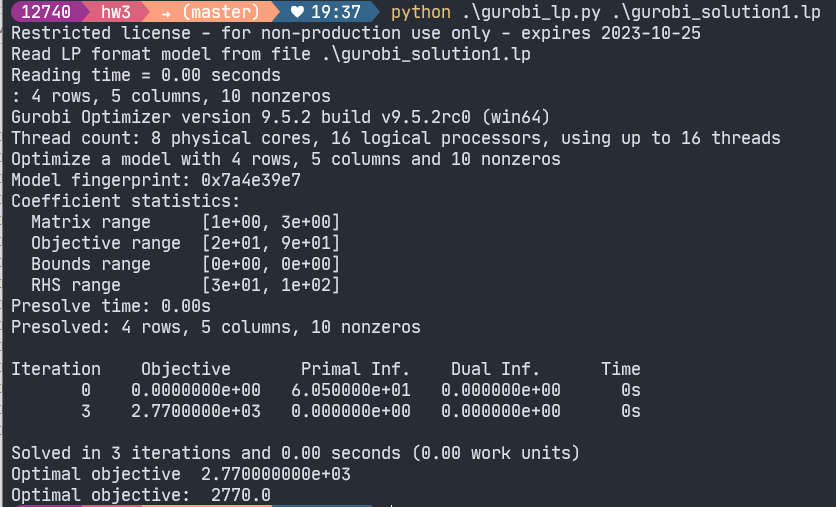
\includegraphics[width=0.9\textwidth]{ans1.png}
    \end{center}
    \caption{}
    \label{fig:ans1}
\end{figure}

\subsubsection{问题2}

\begin{python}
    Min
    20 x0 + 90 x1 + 80 x2 + 70 x3 + 30 x4
    Subject To
        x0 + x1 + x4 >= 30.5
        x2 + x3 >= 30
        3 x0 + 2 x2 <= 120
        3 x1 + 2 x3 + x4 <= 48

    Bounds
    x0 >= 0
    x1 >= 0
    x2 >= 0
    x3 >= 0
    x4 >= 0

    Integer
    x0 x1

    End
\end{python}

求解结果如图\ref{fig:ans2}

\begin{figure}[H]
    \begin{center}
        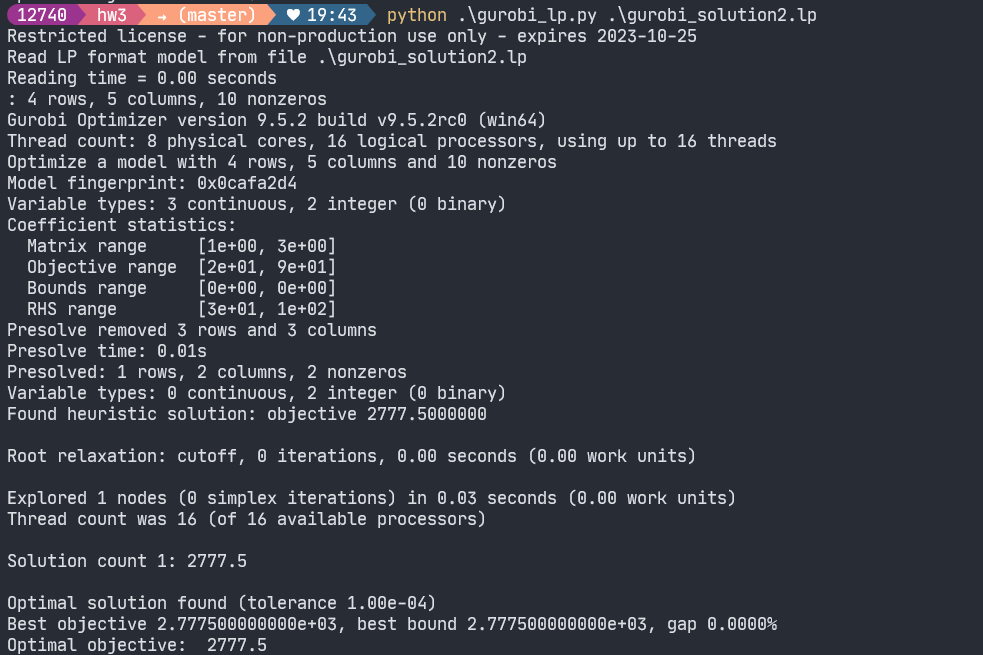
\includegraphics[width=0.9\textwidth]{ans2.png}
    \end{center}
    \caption{}
    \label{fig:ans2}
\end{figure}

\subsubsection{问题3}

\begin{python}
    Min
    20 x0 + 90 x1 + 400 x2 + 70 x3 + 30 x4
    Subject To
        x0 + x1 + x4 >= 30.5
        5 x2 + x3 >= 30
        3 x0 + 10 x2 <= 120
        3 x1 + 2 x3 + x4 <= 48

    Bounds
    x0 >= 0
    x1 >= 0
    x2 >= 0
    x3 >= 0
    x4 >= 0

    Integer
    x0 x1 x2

    End
\end{python}

求解结果如图\ref{fig:ans3}

\begin{figure}[H]
    \begin{center}
        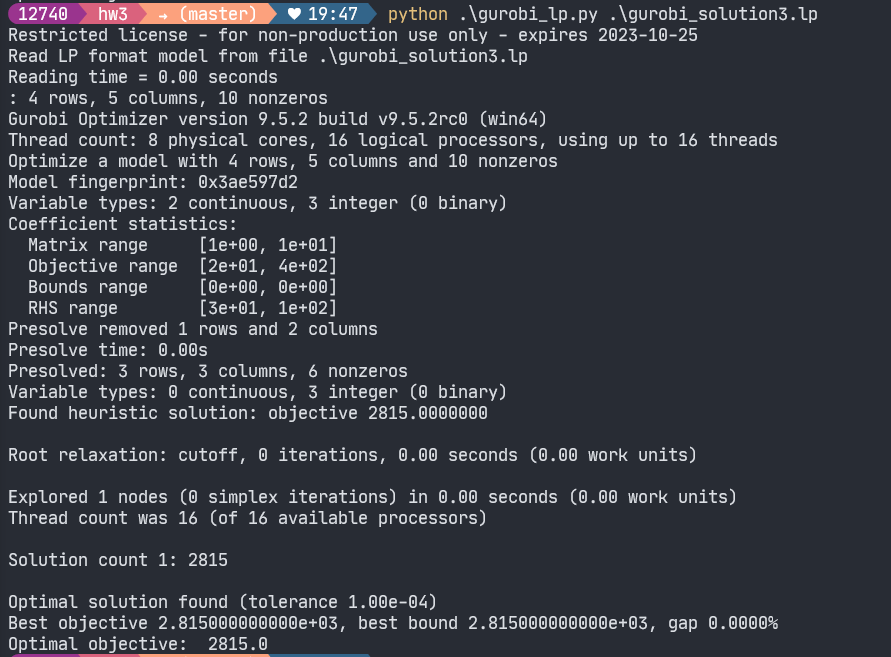
\includegraphics[width=0.9\textwidth]{ans3.png}
    \end{center}
    \caption{}
    \label{fig:ans3}
\end{figure}

